% !TEX root = slides.tex
\usetikzlibrary{positioning,arrows,shapes,shadows}
\tikzstyle{format} = [draw, very thick,color=black, fill=blue!40]
\tikzstyle{medium} = [ellipse, draw, thin, color=black, fill=green!20]
\tikzstyle{qoi}=[rectangle, draw=black, rounded corners, fill=green, drop shadow]
\tikzstyle{cblue}=[circle, draw, thin,fill=blue!10, scale=0.8]
\tikzstyle{decision} = [diamond, draw, thin,color=black,fill=blue!20,
    text width=5.5em, text badly centered, node distance=3cm, inner sep=0pt]
    \tikzstyle{biggray}=[rectangle, draw=black, thin, fill=gray!20,
                                 anchor=south east, text width=14em,
                                 text height=11em, minimum width=0.14em,
                                 minimum height=0.14em, rounded
                                 corners=20pt]

\pgfdeclarelayer{background}
\pgfdeclarelayer{foreground}
\pgfsetlayers{background,main,foreground}

\begin{frame}[t]
\label{sketch}
\frametitle{Forward and Inverse UQ in a workflow}

\centering
\scalebox{0.6}{
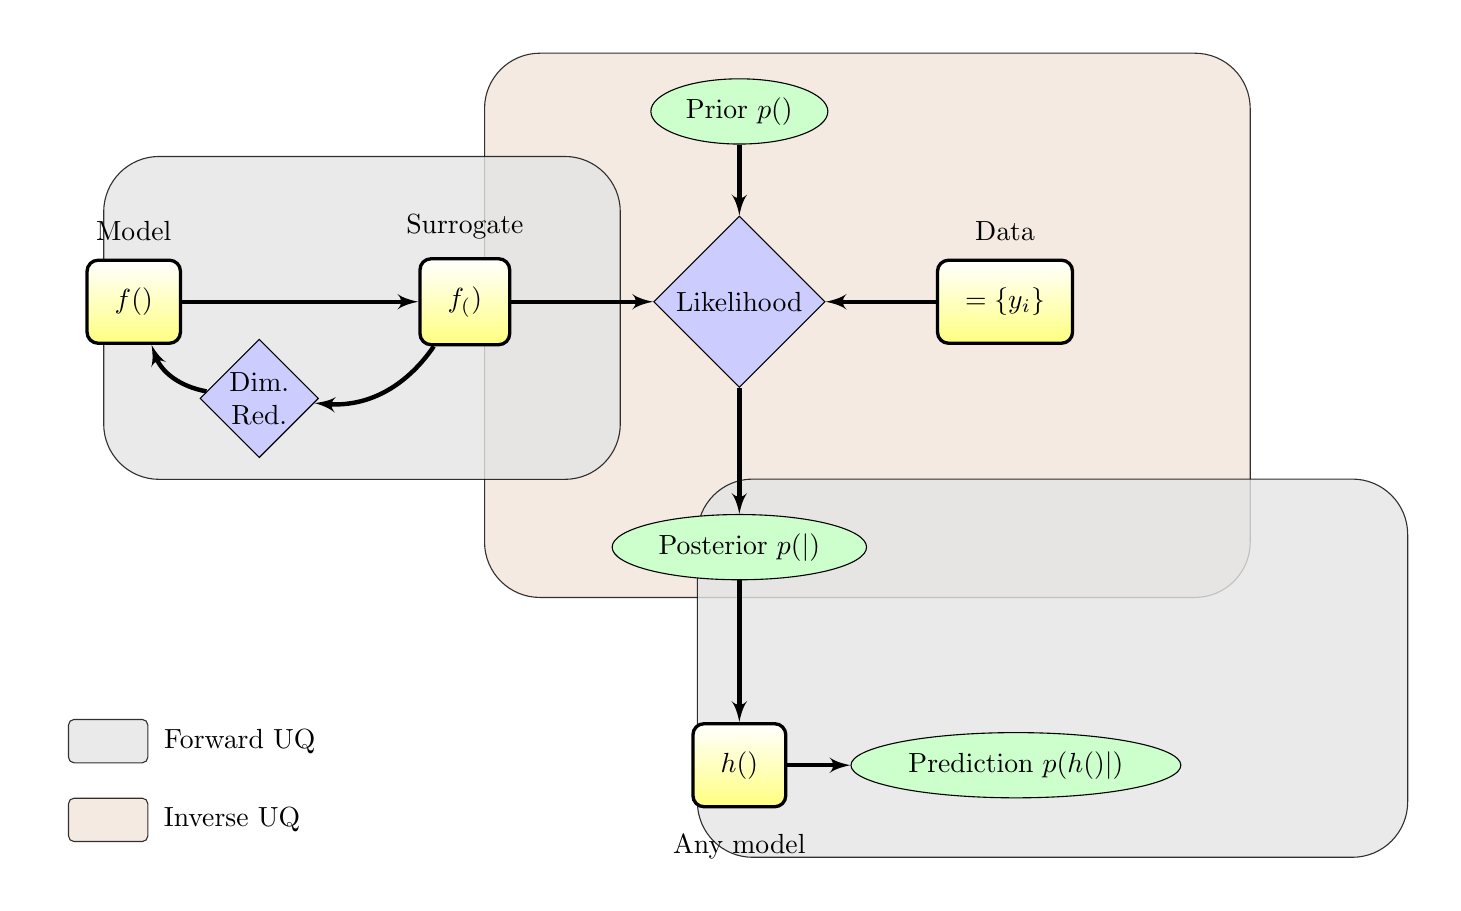
\begin{tikzpicture}[node distance=3cm, auto, thick]
\tikzset{
    mynode/.style={rectangle,rounded corners,draw=black, top color=white, bottom color=yellow!50,very thick, inner sep=1em, minimum size=3em, text centered,color=black},
    mynode2/.style={rectangle,rounded corners,draw=black, top color=white, bottom color=green!50,very thick, inner sep=1em, minimum size=3em, text centered,color=black},
    myarrow/.style={->, >=latex', shorten >=0pt, color=black,ultra thick},
    mylabel/.style={text width=7em,color=black, text centered}
}
    % We need to set at bounding box first. Otherwise the diagram
    % will change position for each frame.
    %\path[use as bounding box] (0,0) rectangle (16,8);
\path[->] node[biggray, fill=gray!20, opacity=0.8, text width=2.2em, text height=0.9em,rounded
                         corners=2pt] at (4,-2.5) (fleg) {};
\path[->] node[biggray, fill=brown!20, opacity=0.8, text width=2.2em, text height=0.9em,rounded
                         corners=2pt] at (4,-3.5) (ileg) {};
\path[->]  node[mylabel, right=-0.2 of fleg](fleet){Forward UQ};
\path[->]  node[mylabel, right=-0.3 of ileg](ilegt){Inverse UQ};


\path[->] node[biggray, fill=brown!20, opacity=0.8, text width=27em, text height=19em] at (18.0,-0.4) (ipred) {};
\path[->] node[biggray, opacity=0.8,text width=18em] at (10,1.1) (cmod) {};
\path[->] node[biggray, opacity=0.8, text width=25em, text height=13em] at (20.0,-3.7) (fpred) {};

\path[->] node[mynode, above right=-2.4 and -6.8 of cmod] (model) {$f(\vlam)$}
               		node[mylabel, above=0.1 of model](model_label){Model};
    	    \path[->] node[mynode, right=3.0 of model] (sur) {$f_\vc(\vlam)$}
        		node[mylabel, above=0.1 of sur](sur_label){Surrogate}
        		%node[mylabel, below=0.1 of fi](fipi){$\pi_\vf(\cdot;\valpha)$}
                  (model) edge [myarrow] (sur);
    \path[->] node[decision, below right=0.3 and 0.6 of model,text width=2.4em] (dred) {Dim. Red.}
                  (sur) edge [myarrow, bend left]  (dred)
                  (dred) edge [myarrow, bend left]  (model);
  \path[->] node[decision, right=1.8 of sur] (xds) {Likelihood}
                  (sur) edge [myarrow]  (xds);
    \path[->] node[mynode, right=1.4 of xds] (gs) {$\DD=\{y_i\}$}
        		node[mylabel, above=0.1 of gs](cmx){Data}
                  (gs) edge [myarrow]  (xds);
   \path[->] node[medium, below=1.6 of xds] (ds) {Posterior $p(\vlam|\DD)$}
                  (xds) edge [myarrow] (ds);
      \path[->] node[medium, above=0.9 of xds] (prior) {Prior $p(\vlam)$}
                  (prior) edge [myarrow] (xds);
       \path[->] node[mynode, below=1.8 of ds] (amodel) {$h(\vlam)$}
            		node[mylabel, below=0.2 of amodel, text width=13em](amodel_label){Any model}
		                         (ds) edge [myarrow]  (amodel);
 \path[->] node[medium, right=0.8 of amodel] (ppred) {Prediction $p(h(\vlam)|\DD)$}
                  (amodel) edge [myarrow] (ppred);

  \begin{pgfonlayer}{background}
    \path (cmod.west |- ipred.north)+(-0.2,0.2) node (a) {};
    \path (fpred.east |- fpred.south)+(+0.2,-0.2) node (b) {};
    %\path[fill=blue!50!green!40!white, opacity=0.6,rounded corners]  (a) rectangle (b); 
    \path[fill=white, opacity=0.6,rounded corners]  (a) rectangle (b); 
    %\path[draw, black, ultra thick, rounded corners]  (a) rectangle (b); 
\end{pgfonlayer}

  \end{tikzpicture}
  }
\end{frame}

